\documentclass[conference]{IEEEtran}
% \IEEEoverridecommandlockouts
% The preceding line is only needed to identify funding in the first footnote. If that is unneeded, please comment it out.
% Template version as of 6/27/2024

\usepackage{cite}
\usepackage{amsmath,amssymb,amsfonts}
\usepackage{graphicx}
\usepackage{textcomp}
\usepackage{xcolor}
\usepackage{tikz}
\usepackage{hyperref}
\usepackage{algorithm}
\usepackage{algpseudocode}

\usetikzlibrary{automata, positioning}
\tikzset{
->, % makes the edges directed
>=stealth, % makes the arrow heads bold
node distance=1.7cm, % specifies the minimum distance between two nodes. Change if necessary.
every state/.style={thick}, % sets the properties for each ’state’ node
initial text=$ $, % sets the text that appears on the start arrow
}

\def\BibTeX{{\rm B\kern-.05em{\sc i\kern-.025em b}\kern-.08em
    T\kern-.1667em\lower.7ex\hbox{E}\kern-.125emX}}
\graphicspath{
    {img/}
}

\begin{document}

\title{An Implementation of Product Construction on Deterministic Finite Automata in Python}

\author{
\IEEEauthorblockN{Evan Childers}
\IEEEauthorblockA{
\textit{University of Alabama}\\
Tuscaloosa, Alabama, United States \\
epchilders@crimson.ua.edu}
\and
\IEEEauthorblockN{August Connors}
\IEEEauthorblockA{
\textit{University of Alabama}\\
Tuscaloosa, Alabama, United States \\
ahconnors@crimson.ua.edu}
\and
\IEEEauthorblockN{Kai NeSmith}
\IEEEauthorblockA{
\textit{University of Alabama}\\
Tuscaloosa, Alabama, United States \\
klnesmith@crimson.ua.edu}
}

\maketitle

\begin{abstract}
In this paper, we discuss the theory and implementation of product construction between two deterministic finite automata (DFAs). In doing so, we discuss the creation of a DFA data structure, the product construction algorithm itself and methods of verifying the product logic through experimentation and visual mediums. We also discuss additional related topics including identifying potentially unreachable states in a resultant DFA as well as the distinction between the intersection and union operations and how they affect the accepting state set.
\end{abstract}

\section{Introduction}
In automata theory, product construction describes the method by which two DFAs are combined into a single DFA to accept a language that is derived from a certain boolean operation on the languages of the original DFAs such as intersection and union. This method plays a pivotal role in many applications in computing theory and formal language processing. In particular, product construction provides a means for which relationships between regular languages can be explored. By constructing a product DFA, one can effectively evaluate whether two DFAs accept overlapping inputs, meet certain logical requirements, or satisfy a desired system behavior.

\section{Problem Statement}
While the process of DFA product construction is a well understood concept in automata theory, the manual computation of a product DFA can become extremely complex and error-prone as the size of the DFAs involved increase. Additionally, the intricacy of these product DFAs can often complicate the process of verifying logical operations like the intersection and union of different automata. This sparks the need for a programmatic solution capable of systematically identifying the product states and transitions, simulating the traversal of a DFA given an input string and presenting the resulting automaton in a clear and interpretable form. This work addresses the lack of available resources regarding this issue by detailing the implementation and formal proof for product construction in Python, along with its potential use cases in verifying logical expressions.

\section{Implementation}
The implementation of the product construction for two deterministic finite automata (DFAs) was developed in Python, utilizing a custom DFA class to encapsulate the automaton’s components and facilitate the construction process. In the scope of this paper, the case of both input DFAs sharing an alphabet was considered for simplicity. The DFA class is initialized with a constructor that accepts five parameters: a list of states, a list of alphabet symbols, a dictionary of transitions mapping state-symbol pairs to destination states, an initial state, and a list of accepting states. This structured representation ensures efficient access to DFA components, simplifying the product construction and state reachability analysis. For the discussion of the product algorithm, the input DFAs will be represented by the tuples
\[ D_1 = (Q_1, \Sigma_1, \delta_1, s_1, F_1) \]
\[ D_2 = (Q_2, \Sigma_2, \delta_2, s_2, F_2) \]
and the product DFA represented by
\[ D' = (Q', \Sigma', \delta', s', F') \]
where $Q$ denotes the list of states, $\Sigma$ the alphabet, $\delta$ the transition function, $s$ the start state, and $F$ the list of accepting states. 

The product construction function is primarily based on the formal definition, particularly adapted from Sipser's interpretation for union \cite{b1}. The function takes two DFA objects as input and generates a new DFA representing either the intersection or union of their languages. In addition to the two DFAs, the function's input includes a flag indicating whether the intersection or union is desired. The function constructs the state set of the product DFA as the Cartesian product of the input DFAs’ state lists, forming pairs $(q_1, q_2)$ where $q_1 \in Q_1, q_2 \in Q_2$. The alphabet is inherited from the input DFAs, as both share the same alphabet. The transition function is defined using the input DFAs’ transition dictionaries: for a state pair $(q_1, q_2) \in Q'$ and symbol $a$, the transition is to $(\delta_1[(q_1, a)], \delta_2[(q_2, a)])$. The initial state of the product DFA is the pair $(s_1, s_2)$. The list of accepting states is the only attribute that differs in the product DFA based on the intersection/union flag. For an intersection, the accepting states are pairs $(q_1, q_2)$ where $q_1 \in F_1$ and $q_2 \in F_2$. For a union, the accepting states are pairs $(q_1, q_2)$ where $q_1 \in F_1$ or $q_2 \in F_2$. These components are then assembled into a new DFA object, leveraging the class’s structured format. The psuedocode for this function is provided in Algorithm \ref{alg:product}.

\begin{algorithm}
\caption{Product Construction of Two DFAs}
\label{alg:product}
\begin{algorithmic}
\State $\Sigma' \gets \Sigma_1$
\State $s' \gets s_1 + "," + s_2$
\For{$q_1 \in Q_1$}
    \For{$q_2 \in Q_2$}
        \State $q' \gets q_1 + "," + q_2$
        \State $Q'.\text{append}(q')$
        \If{intersection}
            \If{$q_1 \in F_1$ and $q_2 \in F_2$}
                \State $F'.\text{append}(q')$
            \EndIf
        \EndIf
        \If{union}
            \If{$q_1 \in F_1$ or $q_2 \in F_2$}
                \State $F'.\text{append}(q')$
            \EndIf
        \EndIf
        \For{$a \in \Sigma'$}
            \State $q_t \gets \delta_1[(q_1, a)] + "," + \delta_2[(q_2, a)]$
            \State $\delta'[(q', a)] \gets q_t$
        \EndFor
    \EndFor
\EndFor
\State \Return \text{DFA}$(Q', \Sigma', \delta', s', F')$
\end{algorithmic}
\end{algorithm}

To identify unreachable states in the product DFA, a breadth-first search (BFS) algorithm was implemented. Starting from the initial state pair, the BFS explores reachable state pairs by iterating over the alphabet and querying the transition dictionary. A queue manages states to be visited, and a set tracks visited states to avoid cycles. If a state returned by the querying of the transition dictionary is not already in the visited states set, it is added to both this set and the queue. The BFS algorithm keeps searching until the queue is empty. At the end of the search, the BFS has compiled a list of reachable states, and any state pairs in the product DFA’s state set not visited are identified as unreachable. This list of unreachable states is output alongside the product DFA, providing insight into the automaton’s structure without modifying its state set.

This implementation benefits from the DFA class’s clear organization, which streamlines the product construction and enables efficient BFS-based analysis, ensuring accurate computation of the DFA product and identification of unreachable states.

\section{Experiments}
In this section, we will explore how product construction can be applied to a variety of different DFAs with a focus on the differences between intersection and union as well as identifying the causes of unreachable states in the resulting automaton

\subsection{Experiment 1}
In this experiment, we started with two DFAs to product construct in order to test the basic capabilities of our implementation. The first DFA, whose transition table is shown in Table \ref{table-exp1-dfa1} and diagram shown in Fig. \ref{fig-exp1-dfa1}, accepts the language that contains strings of length at least two that have a 1 in their second position.

\begin{table}[h!]
    \caption{Experiment 1's DFA 1 Transition Table}
    \begin{displaymath}
        \begin{array}{r|c|c|}
        & 0 & 1 \\
        \hline
        \rightarrow a_0 & a_1 & a_1 \\
        a_1 & a_r & a_2 \\
        * a_2 & a_2 & a_2 \\
        a_r & a_r & a_r \\
        \end{array}
    \end{displaymath}
    \label{table-exp1-dfa1}
\end{table}
\begin{figure}[h!]
    \centering
    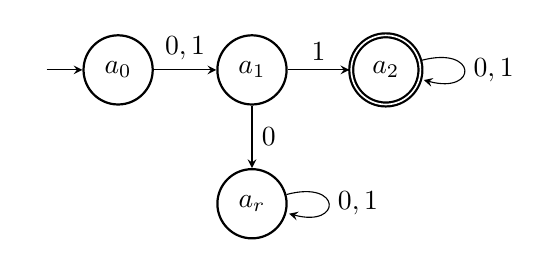
\begin{tikzpicture}
        \node[state, initial] (a0) {$a_{0}$};
        \node[state, right of=a0] (a1) {$a_{1}$};
        \node[state, right of=a1, accepting] (a2) {$a_{2}$};
        \node[state, below of=a1] (areject) {$a_{r}$};
    
        \draw (a0) edge[above] node{$0,1$} (a1)
              (a1) edge[above] node{$1$} (a2)
                   edge[right] node{$0$} (areject)
              (a2) edge[loop right] node{$0,1$} (a2)
              (areject) edge[loop right] node{$0,1$} (areject);
    \end{tikzpicture}
    \caption{Experiment 1's DFA 1}
    \label{fig-exp1-dfa1}
\end{figure}

The second DFA, whose transition table is shown in Table \ref{table-exp1-dfa2} and diagram shown in Fig. \ref{fig-exp1-dfa2}, accepts the language that contains strings that contain at least one 0.

\begin{table}[h!]
    \caption{Experiment 1's DFA 2 Transition Table}
    \begin{displaymath}
        \begin{array}{r|c|c|}
        & 0 & 1 \\
        \hline
        \rightarrow b_0 & b_1 & b_0 \\
        * b_1 & b_1 & b_1 \\
        \end{array}
    \end{displaymath}
    \label{table-exp1-dfa2}
\end{table}
\begin{figure}[h!]
    \centering
    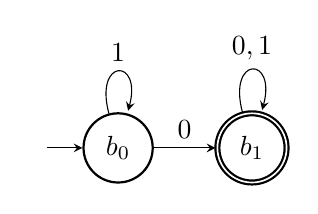
\begin{tikzpicture}
        \node[state, initial] (b0) {$b_{0}$};
        \node[state, right of=b0, accepting] (b1) {$b_{1}$};

        \draw (b0) edge[above] node{$0$} (b1)
                   edge[loop above] node{$1$} (b0)
              (b1) edge[loop above] node{$0,1$} (b1);
    \end{tikzpicture}
    \caption{Experiment 1's DFA 2}
    \label{fig-exp1-dfa2}
\end{figure}

When computing the product of these two DFAs, the resulting transition table is shown in Table \ref{table-exp1-dfaprod} and diagram shown in Fig. \ref{fig-exp1-dfaprod}.

\begin{table}[h!]
    \caption{Experiment 1's Product DFA Transition Table}
    \begin{displaymath}
        \begin{array}{r|c|c|}
        & 0 & 1 \\
        \hline
        \rightarrow a_0,b_0 & a_1,b_1 & a_1,b_0 \\
        a_0,b_1 & a_1,b_1 & a_1,b_1 \\
        a_1,b_0 & a_r,b_1 & a_2,b_0 \\
        a_1,b_1 & a_r,b_1 & a_2,b_1 \\
        a_2,b_0 & a_2,b_1 & a_2,b_0 \\
        * a_2,b_1 & a_2,b_1 & a_2,b_1 \\
        a_r,b_0 & a_r,b_1 & a_r,b_0 \\
        a_r,b_1 & a_r,b_1 & a_r,b_1 \\
        \end{array}
    \end{displaymath}
    \label{table-exp1-dfaprod}
\end{table}
\begin{figure}[h!]
    \centering
    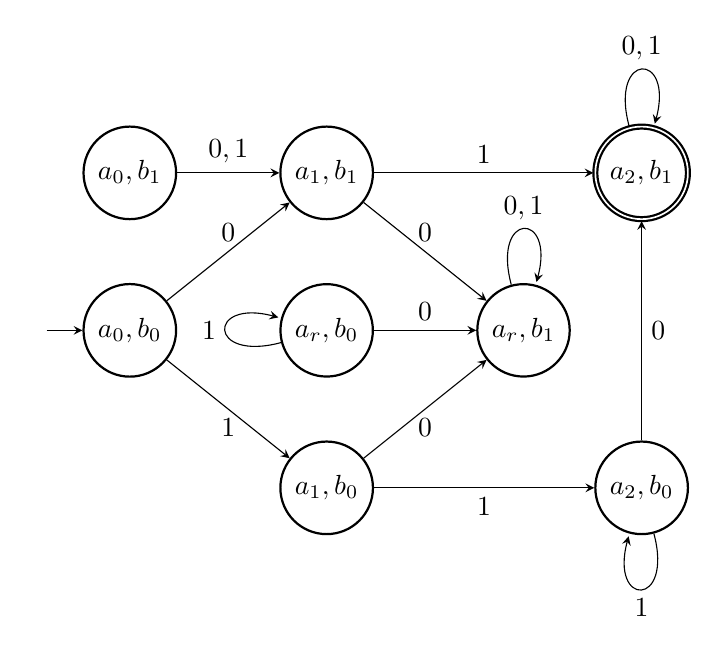
\begin{tikzpicture}
        \node[state, initial] at (0,-2) (a0b0) {$a_0,b_0$};
        \node[state] (a0b1) at (0,0) {$a_0,b_1$};
        \node[state] (a1b0) at (2.5,-4) {$a_1,b_0$};
        \node[state] (a1b1) at (2.5,0) {$a_1,b_1$};
        \node[state] (a2b0) at (6.5,-4) {$a_2,b_0$};
        \node[state, accepting] at (6.5,0) (a2b1) {$a_2,b_1$};
        \node[state] (arb0) at (2.5,-2) {$a_r,b_0$};
        \node[state] (arb1) at (5,-2) {$a_r,b_1$};

        \draw (a0b0) edge[above] node{$0$} (a1b1)
                     edge[below] node{$1$} (a1b0)
              (a0b1) edge[above] node{$0,1$} (a1b1)
              (a1b0) edge[below] node{$0$} (arb1)
                     edge[below] node{$1$} (a2b0)
              (a1b1) edge[above] node{$0$} (arb1)
                     edge[above] node{$1$} (a2b1)
              (a2b0) edge[right] node{$0$} (a2b1)
                     edge[loop below] node{$1$} (a2b0)
              (a2b1) edge[loop above] node{$0,1$} (a2b1)
              (arb0) edge[loop left]  node{$1$} (arb0)
                     edge[above] node {$0$} (arb1)
              (arb1) edge[loop above] node{$0,1$} (arb1);
    \end{tikzpicture}
    \caption{Experiment 1's Product DFA}
    \label{fig-exp1-dfaprod}
\end{figure}

The algorithmically determined unreachable states are \( (a_0, b_1) \) and \( (a_r, b_0) \). When analyzing these state pairs in the context of their original DFAs, we can understand why they are unreachable in the product DFA. For the state pair \( (a_0, b_1) \), note that \( b_1 \) can only be reached from DFA 2's start state by a transition on input 0. However, in DFA 1, \( a_0 \) transitions to a different state on input 0 and does not allow any transitions that lead back to \( a_0 \). Therefore, there is no string that leads to the simultaneous presence of \( a_0 \) and \( b_1 \), rendering this state pair unreachable in the product. A similar rationale applies to \( (a_r, b_0) \). The state \( a_r \) in DFA 1 is reached via a transition on input 0, while \( b_0 \) in DFA 2 transitions away from itself on input 0 and does not return. Thus, there is no string in the input alphabet that can result in the system being in the state \( (a_r, b_0) \), making it unreachable as well.

In order to verify the intersection and union properties, we use the \texttt{accepts\_string} method to test string acceptance in the product DFA. The results, seen in Table \ref{table-exp1-dfabool}, demonstrate the logical operations between the original DFAs.

\begin{table}[h!]
\centering
\caption{Boolean Analysis of Experiment 1's Product DFA Operations}
\label{table-exp1-dfabool}
\begin{tabular}{|c|c|c|c|c|}
\hline
\textbf{DFA Type} & \textbf{11} & \textbf{00} & \textbf{01} & \textbf{1} \\ \hline
DFA 1 & True & False & True & False \\ \hline
DFA 2 & False & True & True & False \\ \hline
Union DFA & True & True & True & False \\ \hline
Intersection DFA & False & False & True & False \\ \hline
\end{tabular}
\end{table} 

As shown in table, the union DFA accepts a string if either original DFA accepts it ($\text{DFA}_1 \cup \text{DFA}_2$), while the intersection DFA only accepts strings accepted by both ($\text{DFA}_1 \cap \text{DFA}_2$). The results confirm the correct implementation of these Boolean operations.

\subsection{Experiment 2}
In this experiment, we started with a pair of slightly larger DFAs in order to further test the capabilities of our product construction implementation. The first DFA, whose transition table is shown in Table \ref{table-exp2-dfa1} and diagram shown in Fig. \ref{fig-exp2-dfa1}, accepts the language that contains strings that have exactly two 0s.

\begin{table}[h!]
    \caption{Experiment 2's DFA 1 Transition Table}
    \begin{displaymath}
        \begin{array}{r|c|c|}
        & 0 & 1 \\
        \hline
        \rightarrow a_0 & a_1 & a_0 \\
        a_1 & a_2 & a_1 \\
        * a_2 & a_3 & a_2 \\
        a_3 & a_3 & a_3 \\
        \end{array}
    \end{displaymath}
    \label{table-exp2-dfa1}
\end{table}
\begin{figure}[h!]
    \centering
    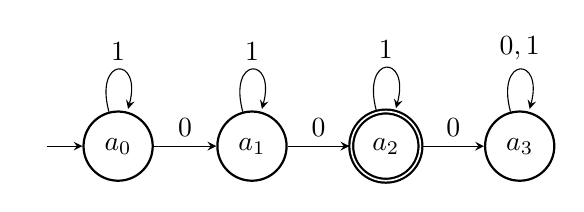
\begin{tikzpicture}
        \node[state, initial] (a0) {$a_{0}$};
        \node[state, right of=a0] (a1) {$a_{1}$};
        \node[state, right of=a1, accepting] (a2) {$a_{2}$};
        \node[state, right of=a2] (a3) {$a_{3}$};
    
        \draw (a0) edge[above] node{$0$} (a1)
                   edge[loop above] node{$1$} (a0)
              (a1) edge[above] node{$0$} (a2)
                   edge[loop above] node{$1$} (a1)
              (a2) edge[above] node{$0$} (a3)
                   edge[loop above] node{$1$} (a2)
              (a3) edge[loop above] node{$0,1$} (a3);
    \end{tikzpicture}
    \caption{Experiment 2's DFA 1}
    \label{fig-exp2-dfa1}
\end{figure}

The second DFA, whose transition table is shown in Table \ref{table-exp2-dfa2} and diagram shown in Fig. \ref{fig-exp2-dfa2}, accepts the language that contains strings that contains at least two 1s.

\begin{table}[h!]
    \caption{Experiment 2's DFA 2 Transition Table}
    \begin{displaymath}
        \begin{array}{r|c|c|}
        & 0 & 1 \\
        \hline
        \rightarrow b_0 & b_0 & b_1 \\
        b_1 & b_1 & b_2 \\
        * b_2 & b_2 & b_2 \\
        \end{array}
    \end{displaymath}
    \label{table-exp2-dfa2}
\end{table}
\begin{figure}[h!]
    \centering
    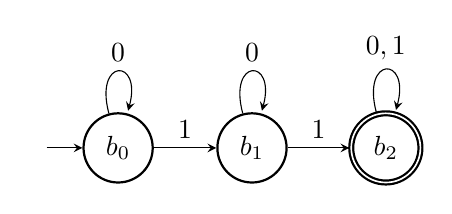
\begin{tikzpicture}
        \node[state, initial] (b0) {$b_{0}$};
        \node[state, right of=b0] (b1) {$b_{1}$};
        \node[state, right of=b1, accepting] (b2) {$b_{2}$};
    
        \draw (b0) edge[above] node{$1$} (b1)
                   edge[loop above] node{$0$} (b0)
              (b1) edge[above] node{$1$} (b2)
                   edge[loop above] node{$0$} (b1)
              (b2) edge[loop above] node{$0,1$} (a2);
    \end{tikzpicture}
    \caption{Experiment 2's DFA 2}
    \label{fig-exp2-dfa2}
\end{figure}

When computing the product of these two DFAs, the resulting transition table is shown in Table \ref{table-exp2-dfaprod} and diagram shown in Fig. \ref{fig-exp2-dfaprod}.

Notably, this experiment differs from Experiment 1 in that it generates no unreachable states, due to the behavior of the two separate DFAs. Since there are only transitions to different states on a 0 input in DFA 1, and only transitions to different states on a 1 input in DFA 2, the resulting product constructed DFA exhibits a lattice-like structure, while ensuring that no resultant states are unreachable (this essentially functions like a coordinate grid, meaning that you can reach any resultant state from the start state on an appropriate input since no transitions in the original DFAs preempt another transition).

\begin{table}[h!]
    \caption{Experiment 2's Product DFA Transition Table}
    \begin{displaymath}
        \begin{array}{r|c|c|}
        & 0 & 1 \\
        \hline
        \rightarrow a_0,b_0 & a_1,b_0 & a_0,b_1 \\
        a_0,b_1 & a_1,b_1 & a_0,b_2 \\
        a_0,b_2 & a_1,b_2 & a_0,b_2 \\
        a_1,b_0 & a_2,b_0 & a_1,b_1 \\
        a_1,b_1 & a_2,b_1 & a_1,b_2 \\
        a_1,b_2 & a_2,b_2 & a_1,b_2 \\
        a_2,b_0 & a_3,b_0 & a_2,b_1 \\
        a_2,b_1 & a_3,b_1 & a_2,b_2 \\
        * a_2,b_2 & a_3,b_2 & a_2,b_2 \\
        a_3,b_0 & a_3,b_0 & a_3,b_1 \\
        a_3,b_1 & a_3,b_1 & a_3,b_2 \\
        a_3,b_2 & a_3,b_2 & a_3,b_2 \\
        \end{array}
    \end{displaymath}
    \label{table-exp2-dfaprod}
\end{table}
\begin{figure}[h!]
    \centering
    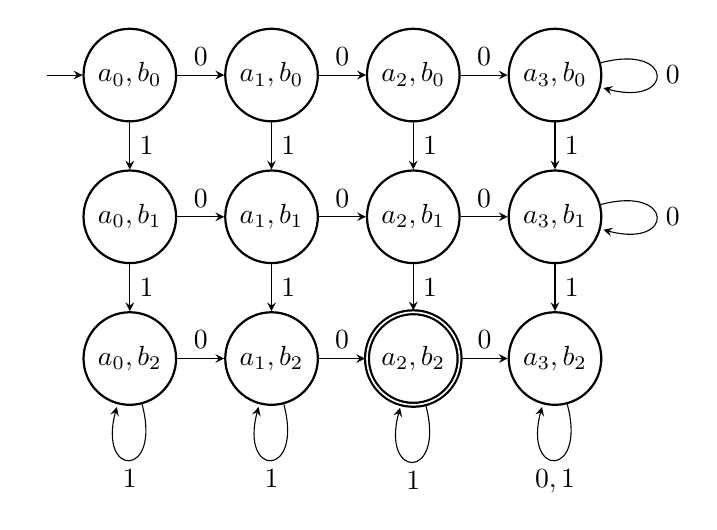
\begin{tikzpicture}
        \node[state, initial] at (0,0) (a0b0) {$a_0,b_0$};
        \node[state] (a0b1) at (0,-1.8) {$a_0,b_1$};
        \node[state] (a0b2) at (0,-3.6) {$a_0,b_2$};
        \node[state] (a1b0) at (1.8,0)  {$a_1,b_0$};
        \node[state] (a1b1) at (1.8,-1.8) {$a_1,b_1$};
        \node[state] (a1b2) at (1.8,-3.6) {$a_1,b_2$};
        \node[state] (a2b0) at (3.6,0)  {$a_2,b_0$};
        \node[state] (a2b1) at (3.6,-1.8) {$a_2,b_1$};
        \node[state, accepting] (a2b2) at (3.6,-3.6) {$a_2,b_2$};
        \node[state] (a3b0) at (5.4,0)  {$a_3,b_0$};
        \node[state] (a3b1) at (5.4,-1.8) {$a_3,b_1$};
        \node[state] (a3b2) at (5.4,-3.6) {$a_3,b_2$};

        \draw (a0b0) edge[above] node{$0$} (a1b0)
                     edge[right] node{$1$} (a0b1)
              (a0b1) edge[above] node{$0$} (a1b1)
                     edge[right] node{$1$} (a0b2)
              (a0b2) edge[above] node{$0$} (a1b2)
                     edge[loop below] node{$1$} (a0b2)
              (a1b0) edge[above] node{$0$} (a2b0)
                     edge[right] node{$1$} (a1b1)
              (a1b1) edge[above] node{$0$} (a2b1)
                     edge[right] node{$1$} (a1b2)
              (a1b2) edge[above] node{$0$} (a2b2)
                     edge[loop below] node{$1$} (a1b2)
              (a2b0) edge[above] node{$0$} (a3b0)
                     edge[right] node{$1$} (a2b1)
              (a2b1) edge[above] node{$0$} (a3b1)
                     edge[right] node{$1$} (a2b2)
              (a2b2) edge[above] node{$0$} (a3b2)
                     edge[loop below] node{$1$} (a2b2)
              (a3b0) edge[loop right] node{$0$} (a3b0)
                     edge[right] node{$1$} (a3b1)
              (a3b1) edge[loop right] node{$0$} (a3b1)
                     edge[right] node{$1$} (a3b2)
              (a3b2) edge[loop below] node{$0,1$} (a3b2);
    \end{tikzpicture}
    \caption{Experiment 2's Product DFA}
    \label{fig-exp2-dfaprod}
\end{figure}

In order to verify the intersection and union properties, we use the \texttt{accepts\_string} method to test string acceptance in the product DFA. The results, seen in Table \ref{table-exp2-dfabool}, demonstrate the logical operations between the original DFAs. As was the case in Experiment 1, the union and intersection DFAs act as expected for the respective operations, thereby supporting our confidence in the implementation.

\begin{table}[h!]
\centering
\caption{Boolean Analysis of Experiment 2's Product DFA Operations}
\label{table-exp2-dfabool}
\begin{tabular}{|c|c|c|c|c|}
\hline
\textbf{DFA Type} & \textbf{000} & \textbf{00} & \textbf{11} & \textbf{0101} \\ \hline
DFA 1 & False & True & False & True \\ \hline
DFA 2 & False & False & True & True \\ \hline
Union DFA & False & True & True & True \\ \hline
Intersection DFA & False & False & False & True \\ \hline
\end{tabular}
\end{table} 

\subsection{Experiment 3}
In this experiment, we started with two DFAs to product construct in order to test and verbosely demonstrate the difference between union and intersection product constructions. As discussed in the Implementation Details section, the only difference between union and intersection operations when performing product construction is the way the accepting states set is constructed. By creating a test to demonstrate this prominently, we would be able to effectively evaluate whether our process successfully constructed the accepting states set. The first DFA, whose transition table is shown in Table \ref{table-exp3-dfa1} and diagram shown in Fig. \ref{fig-exp3-dfa1}, accepts all strings (it is purposefully very simple).

\begin{table}[h!]
    \caption{Experiment 3's DFA 1 Transition Table}
    \begin{displaymath}
        \begin{array}{r|c|c|}
        & 0 & 1 \\
        \hline
        \rightarrow * q_0 & q_0 & q_0 \\
        \end{array}
    \end{displaymath}
    \label{table-exp3-dfa1}
\end{table}
\begin{figure}[h!]
    \centering
    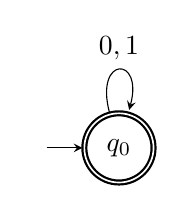
\begin{tikzpicture}
        \node[state, initial, accepting] (q0) {$q_{0}$};
    
        \draw (q0) edge[loop above] node{$0,1$} (q0);
    \end{tikzpicture}
    \caption{Experiment 3's DFA 1}
    \label{fig-exp3-dfa1}
\end{figure}

The second DFA, whose transition table is shown in Table \ref{table-exp3-dfa2} and diagram shown in Fig. \ref{fig-exp3-dfa2}, was designed simply for its complexity; we did not consider the language it accepts, as it is only meant to be dense.

\begin{table}[h!]
    \caption{Experiment 3's DFA 2 Transition Table}
    \begin{displaymath}
        \begin{array}{r|c|c|}
        & 0 & 1 \\
        \hline
        \rightarrow a_0 & a_7 & a_9 \\
        a_1 & a_5 & a_4 \\
        a_2 & a_8 & a_2 \\
        a_3 & a_5 & a_6 \\
        a_4 & a_6 & a_5 \\
        a_5 & a_{10} & a_7 \\
        * a_6 & a_8 & a_3 \\
        a_7 & a_2 & a_7 \\
        * a_8 & a_0 & a_{10} \\
        a_9 & a_4 & a_1 \\
        a_{10} & a_{10} & a_2 \\
        \end{array}
    \end{displaymath}
    \label{table-exp3-dfa2}
\end{table}
\begin{figure}[h!]
    \centering
    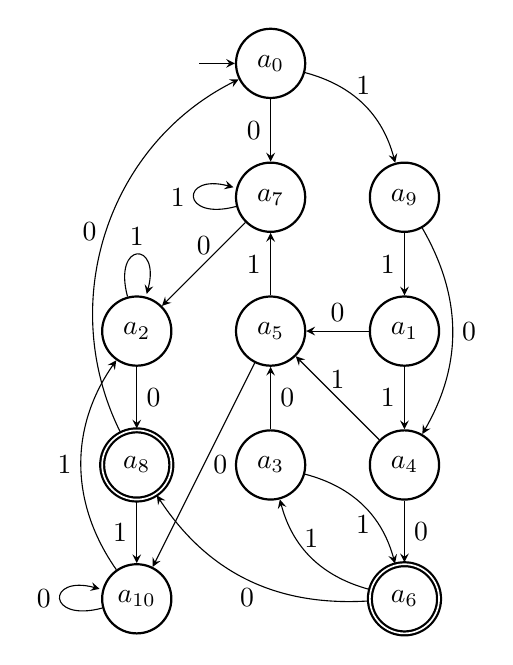
\begin{tikzpicture}
        \node[state, initial] (a0) {$a_{0}$};
        \node[state, below of=a0] (a7) {$a_{7}$};
        \node[state, right of=a7] (a9) {$a_{9}$};
        \node[state, below of=a9] (a1) {$a_{1}$};
        \node[state, below of=a1] (a4) {$a_{4}$};
        \node[state, below of=a7] (a5) {$a_{5}$};
        \node[state, left of=a5] (a2) {$a_{2}$};
        \node[state, accepting, below of=a2] (a8) {$a_{8}$};
        \node[state, below of=a8] (a10) {$a_{10}$};
        \node[state, accepting, below of=a4] (a6) {$a_{6}$};
        \node[state, below of=a5] (a3) {$a_{3}$};
    
        \draw (a0) edge[left] node{$0$} (a7)
                   edge[bend left, above] node{$1$} (a9)
              (a1) edge[above] node{$0$} (a5)
                   edge[left] node{$1$} (a4)
              (a2) edge[right] node{$0$} (a8)
                   edge[loop above] node{$1$} (a2)
              (a3) edge[right] node{$0$} (a5)
                   edge[bend left, below] node{$1$} (a6)
              (a4) edge[right] node{$0$} (a6)
                   edge[above] node{$1$} (a5)
              (a5) edge[right] node{$0$} (a10)
                   edge[left] node{$1$} (a7)
              (a6) edge[bend left, below] node{$0$} (a8)
                   edge[bend left, above] node{$1$} (a3)
              (a7) edge[above] node{$0$} (a2)
                   edge[loop left] node{$1$} (a7)
              (a8) edge[bend left=45, left] node{$0$} (a0)
                   edge[left] node{$1$} (a10)
              (a9) edge[bend left, right] node{$0$} (a4)
                   edge[left] node{$1$} (a1)
              (a10) edge[loop left] node{$0$} (a10)
                   edge[bend left=35, left] node{$1$} (a2);
    \end{tikzpicture}
    \caption{Experiment 3's DFA 2}
    \label{fig-exp3-dfa2}
\end{figure}

When computing the product of these two DFAs using the intersection method (which has been used in the preceding experiments), the resulting transition table is shown in Table \ref{table-exp3-dfaprodi} and diagram shown in Fig. \ref{fig-exp3-dfaprodi}. Note that the transition table and diagram are essentially the same as the original DFA 2. Since DFA 1 is only one state, no "new" states are generated as a result of taking the Cartesian product of the two sets of states (all of DFA 2's states are preserved, just with $q_0$ prepended). Additionally, since we chose to use the intersection method, only state pairs that are both accepting are marked as accepting in the resulting DFA, meaning that DFA 2's original accepting states are also preserved. Therefore, the intersection product DFA is functionally the same as DFA 2.

\begin{table}[h!]
    \caption{Experiment 3's Intersection Product DFA Transition Table}
    \begin{displaymath}
        \begin{array}{r|c|c|}
        & 0 & 1 \\
        \hline
        \rightarrow q_0,a_0 & q_0,a_7 & q_0,a_9 \\
        q_0,a_1 & q_0,a_5 & q_0,a_4 \\
        q_0,a_2 & q_0,a_8 & q_0,a_2 \\
        q_0,a_3 & q_0,a_5 & q_0,a_6 \\
        q_0,a_4 & q_0,a_6 & q_0,a_5 \\
        q_0,a_5 & q_0,a_{10} & q_0,a_7 \\
        * q_0,a_6 & q_0,a_8 & q_0,a_3 \\
        q_0,a_7 & q_0,a_2 & q_0,a_7 \\
        * q_0,a_8 & q_0,a_0 & q_0,a_{10} \\
        q_0,a_9 & q_0,a_4 & q_0,a_1 \\
        q_0,a_{10} & q_0,a_{10} & q_0,a_2 \\
        \end{array}
    \end{displaymath}
    \label{table-exp3-dfaprodi}
\end{table}
\begin{figure}[h!]
    \centering
    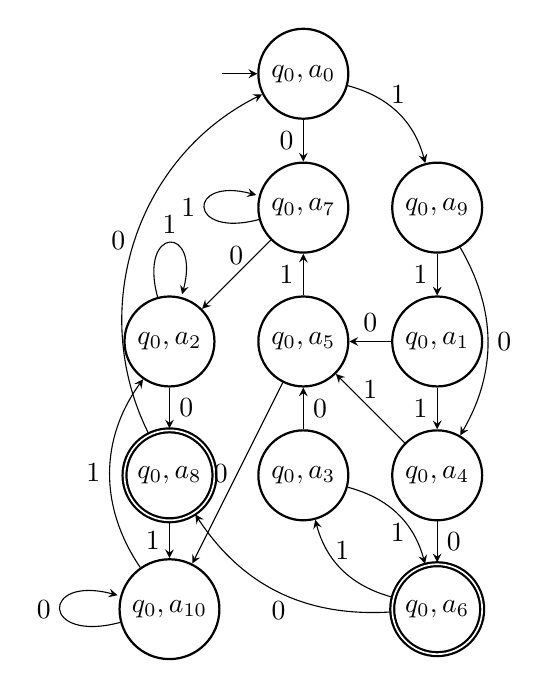
\begin{tikzpicture}
        \node[state, initial] (a0) {$q_0,a_{0}$};
        \node[state, below of=a0] (a7) {$q_0,a_{7}$};
        \node[state, right of=a7] (a9) {$q_0,a_{9}$};
        \node[state, below of=a9] (a1) {$q_0,a_{1}$};
        \node[state, below of=a1] (a4) {$q_0,a_{4}$};
        \node[state, below of=a7] (a5) {$q_0,a_{5}$};
        \node[state, left of=a5] (a2) {$q_0,a_{2}$};
        \node[state, accepting, below of=a2] (a8) {$q_0,a_{8}$};
        \node[state, below of=a8] (a10) {$q_0,a_{10}$};
        \node[state, accepting, below of=a4] (a6) {$q_0,a_{6}$};
        \node[state, below of=a5] (a3) {$q_0,a_{3}$};
    
        \draw (a0) edge[left] node{$0$} (a7)
                   edge[bend left, above] node{$1$} (a9)
              (a1) edge[above] node{$0$} (a5)
                   edge[left] node{$1$} (a4)
              (a2) edge[right] node{$0$} (a8)
                   edge[loop above] node{$1$} (a2)
              (a3) edge[right] node{$0$} (a5)
                   edge[bend left, below] node{$1$} (a6)
              (a4) edge[right] node{$0$} (a6)
                   edge[above] node{$1$} (a5)
              (a5) edge[left] node{$0$} (a10)
                   edge[left] node{$1$} (a7)
              (a6) edge[bend left, below] node{$0$} (a8)
                   edge[bend left, above] node{$1$} (a3)
              (a7) edge[above] node{$0$} (a2)
                   edge[loop left] node{$1$} (a7)
              (a8) edge[bend left=45, left] node{$0$} (a0)
                   edge[left] node{$1$} (a10)
              (a9) edge[bend left, right] node{$0$} (a4)
                   edge[left] node{$1$} (a1)
              (a10) edge[loop left] node{$0$} (a10)
                   edge[bend left=35, left] node{$1$} (a2);
    \end{tikzpicture}
    \caption{Experiment 3's Intersection Product DFA}
    \label{fig-exp3-dfaprodi}
\end{figure}

On the other hand, when computing the product of these two DFAs using the union, the resulting transition table is shown in Table \ref{table-exp3-dfaprodu} and diagram shown in Fig. \ref{fig-exp3-dfaprodu}. Note that once again, as in the intersection case, the states and transitions of DFA 2 are preserved and prepended with $q_0$, but now all states are marked as accepting. This is due to the behavior of DFA 1; since all states in the product DFA contain at least one original accepting state, all states accept via union logic.

\begin{table}[h!]
    \caption{Experiment 3's Union Product DFA Transition Table}
    \begin{displaymath}
        \begin{array}{r|c|c|}
        & 0 & 1 \\
        \hline
        \rightarrow * q_0,a_0 & q_0,a_7 & q_0,a_9 \\
        * q_0,a_1 & q_0,a_5 & q_0,a_4 \\
        * q_0,a_2 & q_0,a_8 & q_0,a_2 \\
        * q_0,a_3 & q_0,a_5 & q_0,a_6 \\
        * q_0,a_4 & q_0,a_6 & q_0,a_5 \\
        * q_0,a_5 & q_0,a_{10} & q_0,a_7 \\
        * q_0,a_6 & q_0,a_8 & q_0,a_3 \\
        * q_0,a_7 & q_0,a_2 & q_0,a_7 \\
        * q_0,a_8 & q_0,a_0 & q_0,a_{10} \\
        * q_0,a_9 & q_0,a_4 & q_0,a_1 \\
        * q_0,a_{10} & q_0,a_{10} & q_0,a_2 \\
        \end{array}
    \end{displaymath}
    \label{table-exp3-dfaprodu}
\end{table}
\begin{figure}[h!]
    \centering
    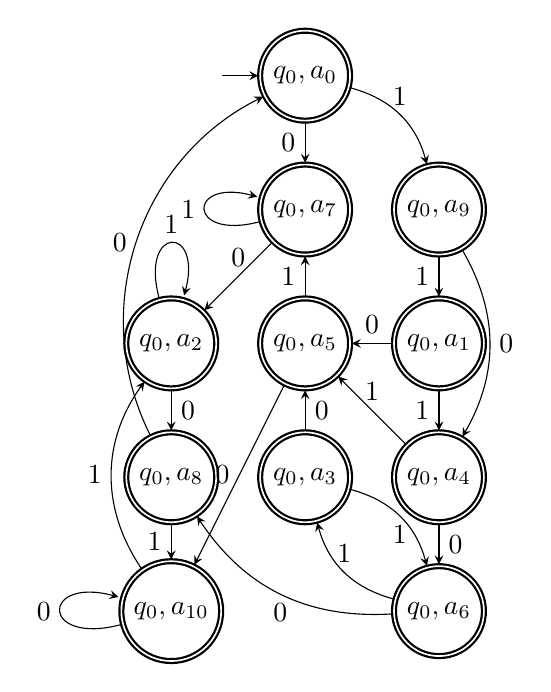
\begin{tikzpicture}
        \node[state, accepting, initial] (a0) {$q_0,a_{0}$};
        \node[state, accepting, below of=a0] (a7) {$q_0,a_{7}$};
        \node[state, accepting, right of=a7] (a9) {$q_0,a_{9}$};
        \node[state, accepting, below of=a9] (a1) {$q_0,a_{1}$};
        \node[state, accepting, below of=a1] (a4) {$q_0,a_{4}$};
        \node[state, accepting, below of=a7] (a5) {$q_0,a_{5}$};
        \node[state, accepting, left of=a5] (a2) {$q_0,a_{2}$};
        \node[state, accepting, below of=a2] (a8) {$q_0,a_{8}$};
        \node[state, accepting, below of=a8] (a10) {$q_0,a_{10}$};
        \node[state, accepting, below of=a4] (a6) {$q_0,a_{6}$};
        \node[state, accepting, below of=a5] (a3) {$q_0,a_{3}$};
    
        \draw (a0) edge[left] node{$0$} (a7)
                   edge[bend left, above] node{$1$} (a9)
              (a1) edge[above] node{$0$} (a5)
                   edge[left] node{$1$} (a4)
              (a2) edge[right] node{$0$} (a8)
                   edge[loop above] node{$1$} (a2)
              (a3) edge[right] node{$0$} (a5)
                   edge[bend left, below] node{$1$} (a6)
              (a4) edge[right] node{$0$} (a6)
                   edge[above] node{$1$} (a5)
              (a5) edge[left] node{$0$} (a10)
                   edge[left] node{$1$} (a7)
              (a6) edge[bend left, below] node{$0$} (a8)
                   edge[bend left, above] node{$1$} (a3)
              (a7) edge[above] node{$0$} (a2)
                   edge[loop left] node{$1$} (a7)
              (a8) edge[bend left=45, left] node{$0$} (a0)
                   edge[left] node{$1$} (a10)
              (a9) edge[bend left, right] node{$0$} (a4)
                   edge[left] node{$1$} (a1)
              (a10) edge[loop left] node{$0$} (a10)
                   edge[bend left=35, left] node{$1$} (a2);
    \end{tikzpicture}
    \caption{Experiment 3's Union Product DFA}
    \label{fig-exp3-dfaprodu}
\end{figure}

The preceding results can be further verified by picking strings that are accepted and using the \texttt{accepts\_string} method to test them using the two product DFAs. The results, seen in Table \ref{table-exp3-dfabool}, demonstrate the logical operations between the original DFAs. Of important note, the table is truncated, as there is no case in which DFA 1 will not accept, so such cases were removed from the table. As can be seen in both the diagrams and from reasoning about the two original DFAs, the union and intersection results are as expected, thereby demonstrating the difference between union and intersection while also verifying an edge case of a singular state.

\begin{table}[h!]
\centering
\caption{Boolean Analysis of Experiment 3's Product DFA Operations}
\label{table-exp3-dfabool}
\begin{tabular}{|c|c|c|}
\hline
\textbf{DFA Type} & \textbf{10010} & \textbf{10011} \\ \hline
DFA 1 & True & True \\ \hline
DFA 2 & False & True \\ \hline
Union DFA & True & True \\ \hline
Intersection DFA & False & True \\ \hline
\end{tabular}
\end{table} 

\section{Contributions}
\subsection{Evan Childers}
For implementation, Evan created the \texttt{accepts\_string} and \texttt{print\_transition\_table} functions, and provided minor fixes to the data cleaning process in the \texttt{read\_dfa\_file} method. He also implemented the \texttt{visualize\_dfa} function, which applies the pre-existing \textit{Automathon} Python library. These functions were used to validate the \texttt{product\_construction} method by writing test cases for the involved DFAs in the \texttt{main} method of the code.\\
Outside of coding, Evan wrote the Introduction and Problem Statement sections of the paper. He also collaborated with Kai to develop and format the Experiments subsection, including the tables and automaton diagrams of the experimental results. He also assisted in writing the Abstract.
\subsection{August Connors}
\textbf{AUGIE CONTRIBUTIONS HERE}
\subsection{Kai NeSmith}
In terms of implementation, Kai created the underlying data structure for handling DFAs in Python, alongside providing the design and saving method for the text file format to read and write DFA data to. They also created and maintained the README file of the repository, improved the main method of the code to allow for command line input, and implemented a GitHub Action that would validate and build the PDF version of this paper in order to validate simultaneous edits.

Outside of code, Kai worked with Evan to test the program by creating experiments and documenting them. In the case of the paper, they formatted the code output into \LaTeX-compatible tables and automaton diagrams in order to deliver a polished final product, while providing the majority of content for Experiments 2 \& 3. They also assisted in writing the conclusion and abstract of the paper.

\section{Conclusion}
In this paper, we described the implementation of a Python-based product construction program which accepts two DFAs as input and produces a product-constructed DFA as output. For the implementation, we developed a basic data structure and built upon it by providing a variety of output options, ranging from the transition table, to a complete text representation, to graphs used to visually check results. We also devised a series of experiments in order to help guide our development and to test the final product and identify problems with the code. In all, we found our implementation to be satisfactory in representing the product construction process, thereby providing a solution to the problem posed to us. The source code repository for this project is available on GitHub: \url{https://github.com/resistiv/CS575-S25-Group3FinalProject}.

% Not sure if we'll need a bibliography, so leaving the template here in case.
\begin{thebibliography}{00}
\bibitem{b1} M. Sipser, \textit{Introduction to the Theory of Computation}. Cengage Learning, 2012.
\bibitem{b2} R. Quintero, “rohaquinlop/automathon,” GitHub, Apr. 04, 2024. https://github.com/rohaquinlop/automathon
\end{thebibliography}

\end{document}
